\chapter{Introduction}
\label{chp:introduction}

While consumer-grade genotyping - such as that used by 23andMe - has proven a popular and inexpensive method to determine Single Nucleotide Polymorphisms (SNPs) in individuals, such methods can only detect a set of reference genes, thus limiting their ability to detect all but the simplest variations.

Whole genome sequencing (without a reference) is a powerful alternative, albeit comparatively expensive. However, the price has been steadily declining: while the Human Genome Project cost \$2.7 billion to complete in 2003~\cite{HGP}, as of 2019 it is possible to have a genome sequenced for \$299~\cite{dantelabscost}, and the price continues to drop.

This decline in price is in large part owed to the advent of Next Generation Sequencing (NGS) machines. The “Sanger” sequencing method used in the Human Genome project required a high degree of human interaction, which NGS machines have subsequently automated, greatly increasing the speed and decreasing the cost. And although NGS machines produce much shorter reads (200 bases versus 800 bases in Sanger sequencing - a human genome is 3.4 billion bases), this is overcome by re-sequencing the same DNA.

%There has been another family of DNA sequencers appearing over the past eight years, which can read an entire chromosome at a time. However, they have unpredictable error profiles, making it difficult to sanitize the data, and it is unlikely this will improve without a major breakthrough in physics (cite). Consequently, instead of replacing NGS machines, they are often used in tandem by providing a reference when combining the short read data that NGS machines produce (cite).

The process of combining short reads into longer sequences is called assembly, and while finding the best overlap is NP-hard~\cite{Mye95}, many practical approaches have been proposed (see surveys \cite{KasMor06, MilKor10, Pop09}).

Traditionally, assembly employed an overlap graph, where each read is a node, and an edge exists if two reads have sufficient overlap~\cite{BatJaf02,HuaYan05,MyeSut00}. Assembly then involves computing a Hamiltonian tour of all nodes. This was an acceptable drawback when dealing with Sanger reads, but is prohibitively expensive to deal with the abundant data that NGS machines produce.

% TODO: Do large k diagram, and single edge diagram

\begin{figure}[!hbt]
	\begin{center}
		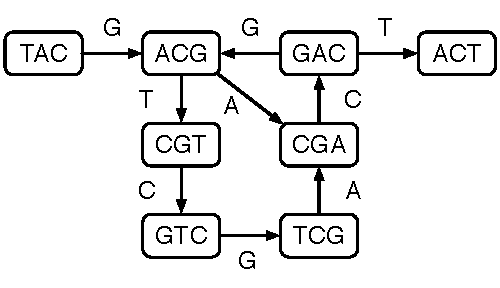
\includegraphics[scale=0.7]{images/dbg.pdf}
		\caption{The $k=3$ de Bruijn graph of strings `TACAC', `TACTC', and
			`GACTC'.}
		\label{figure:dbg}
	\end{center}
\end{figure}

Eulerian assembly~\cite{IW95, PTW} replaces the overlap graph with a de Bruijn graph, where every k-length substring of the reads is a node, and edges represent the k-1 length overlaps, where k is a user selected parameter, as demonstrated in Figure \ref{figure:dbg}. The contigs are then found by finding non-branching paths through this graph. Most modern assembler programs use this paradigm~\cite{bankevich2012spades,peng2010idba,Li:2010,Simpson:2009,Butler:2008,SahShi12,MacPrz09,ZerBir08}. See \cite{compeau11} for a thorough explanation of de Bruijn graphs and their use in assembly.



\begin{figure}[!hbt]
	\begin{center}
		\includegraphics*[scale=0.70]{images/cdbg.pdf}
		\caption{CDBG}
		\label{figure:cdbg}
	\end{center}
\end{figure}


While the de Bruijn graph can be constructed more efficiently than the overlap graph, it remains a bottleneck in assembly, both in terms of speed and size, with a de Bruijn graph of a human genome requiring 300 GB of RAM~\cite{Simpson:2009}. Previous work has reduced this to 30 GB~\cite{Conway}. This thesis reduces this to 2 GB, bringing it in line with commodity hardware - a student or field biologist could now perform this on their laptop. Around the same time as the work done in this thesis, an alternative approach with similar performance was published~\cite{wabi}, but the Burrows-Wheeler approach taken in this thesis offers more flexibility and faster edge traversal.

However, it is common for modern assemblers to build multiple de Bruijn graphs. This is because the k parameter significantly influences the topology - if k is too large, the vertices may not have edges, but if k is too small, the graph can become tangled (diagram). The perfect value of k is different for every set of reads, and in fact, due to non-uniform coverage of NGS data, different areas of the same graph may benefit from differing k values. Hence it has become common practice to build multiple graphs with increasing k, and use them in tandem (cite iterative dbg paper). The work in this thesis bypasses this iterative step, and introduces the first de Bruijn graph that can be built once, yet change k values on-the-fly, at only a modest increase in size over the base succinct de Bruijn graph (mention numbers).

Finally, in population genomics, biologists assemble multiple genomes in order to study the variations (give examples and cite). To avoid constructing multiple graphs, Iqbal et al. proposed the Colored de Bruijn Graph~\cite{ICTFM12}. This graph capitalizes on the fact that DNA is rarely unique to an individual. It does this by first constructing a de Bruijn Graph of the entire populations NGS reads, then, each individual is assigned a unique “color”, and the vertices and edges are annotated with the colors that they belong to. In this thesis, we further augment our succinct de Bruijn Graph to efficiently store these colors. When tested with four plant genomes, Iqbal’s structure required 101 GB RAM, while ours only requires 4 GB of RAM. Furthermore, our structure was able to store all known E. Coli genomes in 42 GB, where Iqbal’s was not able to complete, but is estimated to require 3 TB of RAM. We also demonstrate the use of our structure in creating a database of all Antimicrobial Resistance Genes, requiring 245 GB of RAM (an estimated 18 TB with Iqbal’s structure), for rapidly locating resilient bacterial outbreaks in food supply chains.

These three papers demonstrate that the burrows-wheeler approach is efficient, but can also be augmented to support extra queries that are commonplace in many modern assemblers. Due to the wealth of research on Burrows-Wheeler transforms and Suffix Arrays on which the data
structures in this thesis are based, it is likely that the set of supported operations will continue to grow as applications are found.

\section*{Original Papers}

This thesis is comprised of the following three published papers:

\paragraph{I. Succinct de Bruijn Graphs}

In this paper...

\paragraph{II. Variable-order de Bruijn Graphs}

In this paper...

\paragraph{III. Colored de Bruijn Graphs}

In this paper...
%Sections of this thesis are repeated verbatim from these original published papers:
%<each paper title, where it appeared, and a brief description>.
%Succinct de Bruijn Graphs:
%Variable Order de Bruijn Graphs:
%Succinct Colored de Bruijn Graphs:
%
